%%
%% This is file `sample-sigconf.tex',
%% generated with the docstrip utility.
%%
%% The original source files were:
%%
%% samples.dtx  (with options: `sigconf')
%% 
%% IMPORTANT NOTICE:
%% 
%% For the copyright see the source file.
%% 
%% Any modified versions of this file must be renamed
%% with new filenames distinct from sample-sigconf.tex.
%% 
%% For distribution of the original source see the terms
%% for copying and modification in the file samples.dtx.
%% 
%% This generated file may be distributed as long as the
%% original source files, as listed above, are part of the
%% same distribution. (The sources need not necessarily be
%% in the same archive or directory.)
%%
%%
%% Commands for TeXCount
%TC:macro \cite [option:text,text]
%TC:macro \citep [option:text,text]
%TC:macro \citet [option:text,text]
%TC:envir table 0 1
%TC:envir table* 0 1
%TC:envir tabular [ignore] word
%TC:envir displaymath 0 word
%TC:envir math 0 word
%TC:envir comment 0 0
%%
%%
%% The first command in your LaTeX source must be the \documentclass command.
%\documentclass[sigconf]{acmart}
\documentclass[sigconf,review]{acmart}

\usepackage{enumitem}
\usepackage{color, colortbl}
\usepackage{ragged2e}
\usepackage{array}
\usepackage{amsmath}
\usepackage{listings}
\lstset{
	basicstyle=\ttfamily,
	frame=none,
	breaklines=true,
	numbers=left,
	xleftmargin=2.5em,
	framexleftmargin=0em,
	emphstyle=\textbf,
	float=t
}
\lstdefinestyle{yaml}{
	basicstyle=\ttfamily\small,
	emph={-, :, nsuri, ? }
}

\hyphenation{
	Ex-po-nent-ia-ted-Gra-di-ent-Re-duct-ion
	Ex-po-nent-ia-ted Gra-di-ent Re-duct-ion
	lo-ad pre-proc da-ta a-dult
	Lo-gis-tic-Re-gress-ion
}

%%
%% \BibTeX command to typeset BibTeX logo in the docs
\AtBeginDocument{%
	\providecommand\BibTeX{{%
			\normalfont B\kern-0.5em{\scshape i\kern-0.25em b}\kern-0.8em\TeX}}}

%% Rights management information. This information is sent to you
%% when you complete the rights form. These commands have SAMPLE
%% values in them; it is your responsibility as an author to replace
%% the commands and values with those provided to you when you
%% complete the rights form.
\setcopyright{acmcopyright}
\copyrightyear{2022}
\acmYear{2022}
\acmDOI{XXXXXXX.XXXXXXX}

%% These commands are for a PROCEEDINGS abstract or paper.
\acmConference[MODELS '22]{ACM / IEEE 25th International Conference on Model Driven Engineering Languages and Systems}{October 23--28,
	2022}{Montreal, Canada}
\acmPrice{15.00}
\acmISBN{978-1-4503-XXXX-X/22/10}


%%
%% Submission ID.
%% Use this when submitting an article to a sponsored event. You'll
%% receive a unique submission ID from the organisers
%% of the event, and this ID should be used as the parameter to this command.
%%\acmSubmissionID{123-A56-BU3}

%%
%% The majority of ACM publications use numbered citations and
%% references. The command \citestyle{authoryear} switches to the
%% "author year" style.
%%
%% If you are preparing content for an event
%% sponsored by ACM SIGGRAPH, you must use the "author year" style of
%% citations and references.
%% Uncommenting
%% the next command will enable that style.
%%\citestyle{acmauthoryear}

%%
%% end of the preamble, start of the body of the document source.
\begin{document}
	
	%%
	%% The "title" command has an optional parameter,
	%% allowing the author to define a "short title" to be used in page headers.
	\title{Towards Model-based Bias Mitigation in Machine Learning}
	
	%%
	%% The "author" command and its associated commands are used to define
	%% the authors and their affiliations.
	%% Of note is the shared affiliation of the first two authors, and the
	%% "authornote" and "authornotemark" commands
	%% used to denote shared contribution to the research.
	%\author{Ben Trovato}
	%\authornote{Both authors contributed equally to this research.}
	%\email{trovato@corporation.com}
	%\orcid{1234-5678-9012}
	%\author{G.K.M. Tobin}
	%\authornotemark[1]
	%\email{webmaster@marysville-ohio.com}
	%\affiliation{%
		%  \institution{Institute for Clarity in Documentation}
		%  \streetaddress{P.O. Box 1212}
		%  \city{Dublin}
		%  \state{Ohio}
		%  \country{USA}
		%  \postcode{43017-6221}
		%}
	%
	%\author{Lars Th{\o}rv{\"a}ld}
	%\affiliation{%
		%  \institution{The Th{\o}rv{\"a}ld Group}
		%  \streetaddress{1 Th{\o}rv{\"a}ld Circle}
		%  \city{Hekla}
		%  \country{Iceland}}
	%\email{larst@affiliation.org}
	%
	%\author{Valerie B\'eranger}
	%\affiliation{%
		%  \institution{Inria Paris-Rocquencourt}
		%  \city{Rocquencourt}
		%  \country{France}
		%}
	%
	%\author{Aparna Patel}
	%\affiliation{%
		% \institution{Rajiv Gandhi University}
		% \streetaddress{Rono-Hills}
		% \city{Doimukh}
		% \state{Arunachal Pradesh}
		% \country{India}}
	%
	%\author{Huifen Chan}
	%\affiliation{%
		%  \institution{Tsinghua University}
		%  \streetaddress{30 Shuangqing Rd}
		%  \city{Haidian Qu}
		%  \state{Beijing Shi}
		%  \country{China}}
	%
	%\author{Charles Palmer}
	%\affiliation{%
		%  \institution{Palmer Research Laboratories}
		%  \streetaddress{8600 Datapoint Drive}
		%  \city{San Antonio}
		%  \state{Texas}
		%  \country{USA}
		%  \postcode{78229}}
	%\email{cpalmer@prl.com}
	%
	%\author{John Smith}
	%\affiliation{%
		%  \institution{The Th{\o}rv{\"a}ld Group}
		%  \streetaddress{1 Th{\o}rv{\"a}ld Circle}
		%  \city{Hekla}
		%  \country{Iceland}}
	%\email{jsmith@affiliation.org}
	%
	%\author{Julius P. Kumquat}
	%\affiliation{%
		%  \institution{The Kumquat Consortium}
		%  \city{New York}
		%  \country{USA}}
	%\email{jpkumquat@consortium.net}
	
	\author{Alfa Yohannis}
	\affiliation{%
		\institution{University of York}
		\city{York}
		\country{United Kingdom}}
	\email{alfa.yohannis@york.ac.uk}
	
	\author{Dimitris Kolovos}
	\affiliation{%
		\institution{University of York}
		\city{York}
		\country{United Kingdom}}
	\email{dimitris.kolovos@york.ac.uk}
	
	%%
	%% By default, the full list of authors will be used in the page
	%% headers. Often, this list is too long, and will overlap
	%% other information printed in the page headers. This command allows
	%% the author to define a more concise list
	%% of authors' names for this purpose.
	\renewcommand{\shortauthors}{Yohannis and Kolovos}
	
	%%
	%% The abstract is a short summary of the work to be presented in the
	%% article.
	\begin{abstract}
		Models produced by machine learning are not guaranteed free from bias, particularly when trained and tested with data produced in discriminatory environments. The bias can be unethically acceptable, mainly when the data contains sensitive attributes, such as sex, race, age, etc. Some approaches have contributed to mitigating such biases by providing bias metrics and mitigation algorithms. The challenge is that users have to implement their code in general/statistical programming languages, which can be demanding for users with little programming and fairness in machine learning experience. FairML provides a model-based approach to improve the productivity of bias measurement and mitigation by raising their abstraction and automatically generating their implementation code. Our evaluation shows that FairML requires fewer lines of code to produce similar measurement values, with $pm$ 0.1 tolerance, to the ones made by the baseline code.
	\end{abstract}
	
	%%
	%% The code below is generated by the tool at http://dl.acm.org/ccs.cfm.
	%% Please copy and paste the code instead of the example below.
	%%
	\begin{CCSXML}
		<ccs2012>
		<concept>
		<concept_id>10003752.10010070.10010071.10010083</concept_id>
		<concept_desc>Theory of computation~Models of learning</concept_desc>
		<concept_significance>300</concept_significance>
		</concept>
		<concept>
		<concept_id>10010405.10010455</concept_id>
		<concept_desc>Applied computing~Law, social and behavioral sciences</concept_desc>
		<concept_significance>500</concept_significance>
		</concept>
		<concept>
		<concept_id>10011007.10011006.10011041.10011047</concept_id>
		<concept_desc>Software and its engineering~Source code generation</concept_desc>
		<concept_significance>500</concept_significance>
		</concept>
		<concept>
		<concept_id>10011007.10011006.10011050.10011017</concept_id>
		<concept_desc>Software and its engineering~Domain specific languages</concept_desc>
		<concept_significance>500</concept_significance>
		</concept>
		</ccs2012>
	\end{CCSXML}
	
	\ccsdesc[300]{Theory of computation~Models of learning}
	\ccsdesc[500]{Applied computing~Law, social and behavioral sciences}
	\ccsdesc[500]{Software and its engineering~Source code generation}
	\ccsdesc[500]{Software and its engineering~Domain specific languages}
	%%
	%% Keywords. The author(s) should pick words that accurately describe
	%% the work being presented. Separate the keywords with commas.
	\keywords{Model-Driven Engineering, Generative Programming, Bias Mitigation, Bias Metrics, Machine Learning}
	
	%% A "teaser" image appears between the author and affiliation
	%% information and the body of the document, and typically spans the
	%% page.
	%\begin{teaserfigure}
	%  \includegraphics[width=\textwidth]{sampleteaser}
	%  \caption{Seattle Mariners at Spring Training, 2010.}
	%  \Description{Enjoying the baseball game from the third-base
		%  seats. Ichiro Suzuki preparing to bat.}
	%  \label{fig:teaser}
	%\end{teaserfigure}
	
	%%
	%% This command processes the author and affiliation and title
	%% information and builds the first part of the formatted document.
	\maketitle
	
	\section{Introduction}
	\label{sec:introduction}
	The use of machine learning is pervasive nowadays, from personal daily activities, such as face recognition for authentication and voice processing when talking to intelligent assistants (e.g., Alexa, Siri), to performing sensitive, ethical tasks, such as predicting criminals and classifying profiles for loans. While machine learning does bring efficiency, models produced by machine learning are not guaranteed free from bias, particularly when trained and tested with data produced in discriminatory environments. The tendency can be unacceptable, mainly when it touches sensitive attributes, such as sex, race, age, etc., and cause unfairness. 
	
	In 2016, an algorithm for predicting recidivism was found to produce a high false-negative rate for white people and a high false-positive rate for black people \cite{angwin2016machine}. Some commercial face recognition services were also seen to have significantly lower accuracy on darker-skin females \cite{buolamwini2018gender}. Moreover, A job platform was found to rank qualified female candidates far lower than qualified male candidates even though they have similar properties \cite{lahoti2019ifair}. These are some instances that show biases in machine learning can promote unfairness. 
	
	Some approaches have contributed to the mitigation of such biases by providing bias metrics and debiasing algorithms (more in Sections \ref{sec:bias_metrics} and \ref{sec:bias_mitigation}). 
	Different toolkits have implemented these metrics and algorithms.
	However, they come with different methodological approaches and capabilities, which demand users to understand them before they can decide which toolkits are best for specific scenarios~\cite{lee2021landscape}.  
	
	Data scientists usually work using their intuitions to narrow down the number of combinations of algorithms, parameters, and other factors to find the best models for given goals, datasets, and domains \cite{muller2016introduction}. After that, with lots of experimentation and trial and error \cite{byrne2017development}, they have to go through all the narrowed combinations and test the produced models to identify which models are the best. Moreover, regardless of the availability of machine learning libraries, data scientists have to craft the search process from scratch in general/statistical programming languages (e.g, Python, R).
	
	Model-Driven Sofware Development (MDSE) leverages the abstraction of software development by hiding technical details of implementation that can be automated \cite{brambilla2017model}. Thus, users can focus on essential aspects through the use of simpler modelling languages, and the target implementation can be automatically generated, which in turn improves productivity \cite{volter2013model}. The use of MDSE would benefit data scientists since it allows them to search for the best bias mitigation methods for given cases at a higher abstraction level. They also do not have to code the implementation of the search process in general/statistical programming languages since it can be automatically generated and then fine-tuned later on. 
	
	FairML is a tool that implements the MDSE approach to model and automate bias measurement and mitigation in machine learning. 
	\begin{enumerate}
		\item FairML raises the abstraction of bias measurement and mitigation so that users can configure their bias mitigation model in YAML (YAML Ain't Markup Language), a human-friendly declarative language \cite{evans2017yaml}, without having to code in general/statistical programming languages.
		\item FairML supports a certain degree of expressiveness, allowing users to experiment with different kinds of bias metrics, bias mitigation algorithms, datasets, classifiers, and their parameters to find the best combinations that reduce biases but with acceptable accuracy.
		\item It automatically generates Python and Jupyter Notebook files which users can execute to measure and mitigate biases on given datasets. All generated files are modifiable and extensible for fine-tuning and further development.
	\end{enumerate}
	
	This paper is structured as follows. First, we discuss fairness in machine Learning in Section \ref{sec:bias_in_machine_learning}. The section covers the definitions of some related terms, real examples, bias metrics, and bias mitigation. In Section \ref{sec:model_based_bias_mitigation}, we present an overview of our development as well as our approach to implementing the techniques from the field to automate bias mitigation. 
	%Section \ref{sec:example} 
	The section also presents how users use an existing toolkit in expressing a solution to mitigate bias in classification. We also demonstrate how FairML represents the solution in more readable, shorter lines and can automatically produce generated code with the same correctness as the manually crafted ones.
	In section \ref{sec:evaluation}, we evaluate FairML on expressiveness, correctness, generation time, and execution time and use the existing code of a bias mitigation toolkit as the benchmark. Section \ref{sec:result_and_discussion} presents and discusses the result of the evaluation. 
	We also reflect on some lessons we learned during the research and development of FairML in Section \ref{sec:lessons_learned}. 
	Section \ref{sec:related_work} overview some related work. 
	Finally, Section \ref{sec:conclusions_and_future_work} presents the conclusions and future work of this research.
	
	\section{Bias in Machine Learning}
	\label{sec:bias_in_machine_learning}
	This section briefly discusses fairness in machine learning, which covers the definitions of some related terms, real examples, bias metrics, and bias mitigation.
	
	\subsection{Definitions and Examples}
	\label{sec:definitions_and_examples}
	
	Fairness is defined as ``the absence of any prejudice or favouritism toward an individual or
	group based on their inherent or acquired characteristics'' \cite{mehrabi2021survey}.
	The absence of fairness can be caused by a bias which is a systematic error or distortion from the actual state of affairs due to flaws in data collection and processing, study design, analysis, and interpretation \cite{oxford2022bias}. 
	The unfairness happens when biases put privileged groups in an advantaged position against unprivileged groups \cite{bellamy2018ai}. 
	Bias can also be caused by harmful discrimination if the distinction made is due to intentional or unintentional stereotyping and prejudice based on sensitive attributes (race, age, sex, etc.) \cite{mehrabi2021survey,chen2019fairness}. 
	
	For example, in 2006, it was found that COMPAS, the algorithm used for recidivism prediction, produces a much higher false-positive rate for black people than white people \cite{angwin2016machine}. Another example is XING, a job platform similar to LinkedIn, which was found to rank less qualified male candidates higher than more qualified female candidates \cite{lahoti2019ifair}. The paper states that fairness between female and male groups has been achieved, but group fairness did not necessarily indicate fairness for individuals. Moreover, publicly available commercial face recognition online services provided by Microsoft, Face++, and IBM, respectively, are found to suffer from achieving much lower accuracy on females with darker skin colour \cite{buolamwini2018gender}. There are other examples of biases in machine learning, but these three examples already demonstrate that, in practice, machine learning is not always fair, and the unfairness can bring disadvantages to specific groups. 
	
	
	\subsection{Bias Metrics}
	\label{sec:bias_metrics}
	
	%\begin{figure*}[h]
	%	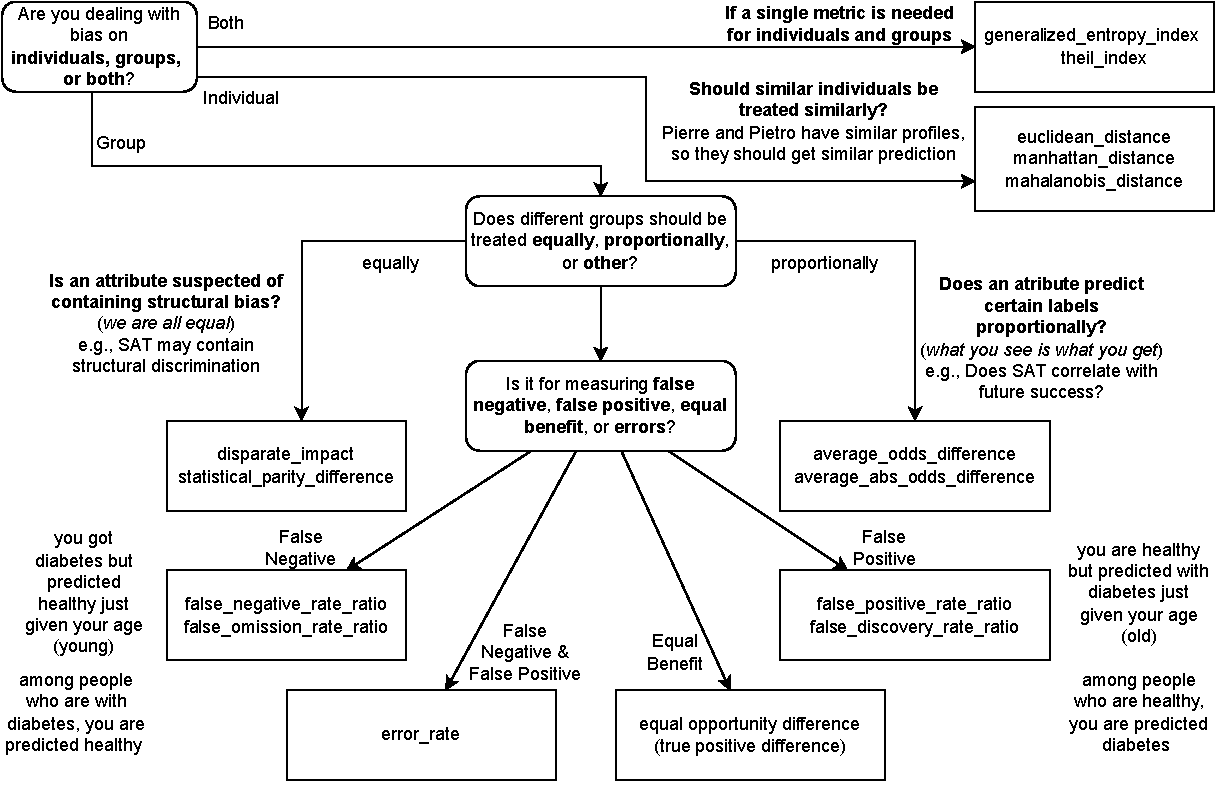
\includegraphics[width=\linewidth]{figures/wizard-metric}
	%	\caption{The decision tree to automatically select the most appropriate bias metrics for particular situations.}
	%	\label{fig:wizard-metric}
	%\end{figure*}
	
	Some metrics have been developed to detect and measure biases in machine learning. Each metric has its way of calculating biases and therefore is preferable to others in particular situations. IBM AI Fairness 360 \cite{mahoney2020ai,ibmaif3602022guidance} and Aequitas\footnote{\url{http://aequitas.dssg.io/static/images/metrictree.png}} have provided guidance for the selection. So, if a bias measurement requires metrics that encompass group and individual fairness, then Theil Index \cite{conceicao2000theyoung,bellamy2018ai} and Generalised Entropy Index \cite{speicher2018unified} are preferable. Theil Index is the generalised entropy index but with alpha equal to 1. They can be used as a unified metric to measure the inequality in benefit allocation for groups and individuals \cite{ibmaif3602022guidance,mahoney2020ai}. Lower scores reflect strong fairness, while the higher ones show the opposite. Perfect fairness is indicated by a value of 0 \cite{lale2022doc}. 
	
	Euclidean Distance, Manhattan Distance, and Mahalanobis Distance are the metrics to measure individual fairness. These metrics are used to measure the distance of the same individual in the original and debiased datasets \cite{bellamy2018ai}. These metrics are required to ensure consistency since data transformation, when applying bias mitigation in pre-processing, can achieve group fairness but might cause unfairness to individuals. The reference \cite{calmon2017optimized} uses these metrics as constraints to limit the distortion of its bias mitigation so that group fairness can be achieved with individual fairness in mind. 
	
	There are two main world views for group fairness: equal and proportional fairness \cite{mahoney2020ai,ibmaif3602022guidance}. Equal fairness means under-represented groups should have a similar chance as the rest regarding prediction results and usually is applied to systems perceived to have structural discrimination. For example, A-level, SAT, or other national exams are suspected to contain structural discrimination. Statistical Parity Difference \cite{dwork2012fairness,mahoney2020ai,ibmaif3602022guidance} and Disparate Impact \cite{feldman2015disparate,mahoney2020ai,ibmaif3602022guidance} are the common metrics to measure equal fairness. 
	
	Statistical Parity Difference is computed as the difference of probabilities of being labelled favourable between the privileged and unprivileged groups (Equation \ref{eq:statistical_parity_difference}) \cite{dwork2012fairness,ibmaif3602022doc,bellamy2018ai}. 
	\begin{equation} \label{eq:statistical_parity_difference}
		SPD = Pr(\hat{Y} = 1 | D = \text{unpriv})
		- Pr(\hat{Y} = 1 | D = \text{priv})
	\end{equation}
	The ideal value of the metric is 0. A negative value implies that the labelling favours the privileged group, while a positive value implies the opposite \cite{ibmaif3602022doc,bellamy2018ai}. Disparate Impact \cite{feldman2015disparate,ibmaif3602022doc,bellamy2018ai} computes fairness as the ratio of probabilities of being labelled favourable between the unprivileged and privileged groups (Equation \ref{eq:disparate_impact}).
	\begin{equation} \label{eq:disparate_impact}
		DI = \frac{Pr(\hat{Y} = 1 | D = \text{unprivileged})}
		{Pr(\hat{Y} = 1 | D = \text{privileged})}
	\end{equation}
	The ideal value of this metric is 1.0. A value $<$ 1 indicates that the labelling advantages the privileged group and a value $>$ 1 disadvantage the unprivileged group \cite{ibmaif3602022doc,bellamy2018ai}.
	
	In contrast, proportional fairness, a.k.a. what you see is what you get (WYSIWYG),  perceives that certain features correlate with certain labels, and therefore the features can be used to predict the labels. For example, the scores of A-level, SAT, or other national exams correlate with incomes in the future \cite{mahoney2020ai,ibmaif3602022guidance}. Average Odds Difference is the metric to measure proportional fairness. The metric computes bias as the average difference of false-positive rate ($FPR = FP/N$, false positives / all negatives) and true positive rate ($TPR = TP/P$, true positives / all positives) between unprivileged and privileged groups (Equation \ref{eq:average_odds_difference}) \cite{ibmaif3602022doc,bellamy2018ai}.
	\begin{equation} \label{eq:average_odds_difference}
		\begin{aligned}
			AOD = \tfrac{1}{2}* ((FPR_{D = \text{unprivileged}} - FPR_{D = \text{privileged}}) +\\
			(TPR_{D = \text{unprivileged}} - TPR_{D = \text{privileged}}))
		\end{aligned}
	\end{equation}
	The ideal value of the metric is 0. A negative value indicates the privileged group is more favourable than the unprivileged group while a positive value indicates the opposite \cite{ibmaif3602022doc,bellamy2018ai}. 
	
	There are also other metrics that fall in between equal and proportional fairness. For example, Equal Opportunity Difference \cite{ibmaif3602022doc,bellamy2018ai} is a metric that calculates bias as the difference of true positive rates between the unprivileged and the privileged groups (Equation \ref{eq:equal_opportunity_difference}). 
	\begin{equation} \label{eq:equal_opportunity_difference}
		EOD = TPR_{D = \text{unprivileged}} - TPR_{D = \text{privileged}}	
	\end{equation}
	The true-positive rate is the ratio of true positives to the total number of all positive outcomes ($TPR=TP/P$) for a given group. The ideal value is 0, and a negative value indicates a higher preference for the privileged group while a positive one is the opposite \cite{ibmaif3602022doc,bellamy2018ai}. Other metrics in this space are False Negative Rate Ratio and Difference, False Omission Rate Ratio and Difference, Error Rate, False Positive Rate Ratio and Difference, and False Discovery Rate Ratio and Difference \cite{mahoney2020ai,ibmaif3602022guidance}.
	
	%\begin{figure*}
	%	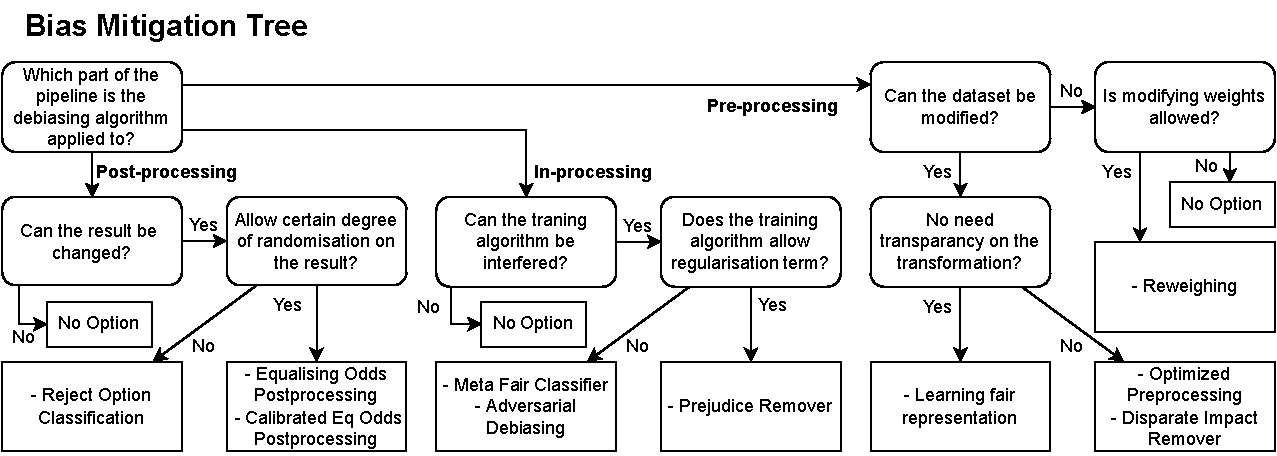
\includegraphics[width=\linewidth]{figures/wizard-debiasing}
	%	\caption{The decision tree to select the most appropriate debiasing algorithms for particular situations.}
	%	\label{fig:wizard-debiasing}
	%\end{figure*}
	
	\subsection{Bias Mitigation}
	\label{sec:bias_mitigation}
	
	Debiasing algorithms have been developed to reduce biases in machine learning, and they can be categorised based on the stages where they are applied in machine learning pipelines: pre-processing, in-processing, and post-processing. References \cite{mahoney2020ai,ibmaif3602022guidance} provide guidances the choose the most appropriate the debiasing algorithms for specific situations.
	
	Reference \cite{mahoney2020ai} recommends to mitigate unfairness as early as possible particularly in the pre-processing stage since biases that are reduced in that stage are intrinsic in datasets. Unfortunately, there are conditions where altering datasets is prohibited. So, if modifying datasets is not allowed, \textbf{Reweighing} \cite{kamiran2011reweighing} can be an option since it does not alter the values of features but works by altering only the weight of each label/prediction to gain fairness. If modifying datasets is allowed, \textbf{Optimized Preprocessing} \cite{calmon2017optimized}, \textbf{Disparate Impact Remover} \cite{feldman2015disparate}, and \textbf{Learning Fair Representation} (LFR) \cite{zemel2013lfr} can be the options except that LFR does not provide transparency since it encodes data into a latent space, and therefore the first two are preferable when transparency of dataset transformation is required.
	Optimized Preprocessing learns a probabilistic transformation that modify the labels and features of a dataset but with objectives and constraints on individual distortion, data fidelity, and group fairness \cite{mahoney2020ai,calmon2017optimized}.
	Disparate Impact Remover alters the values of features to increase the fairness of groups while preserving rank-ordering within groups \cite{mahoney2020ai,feldman2015disparate}.
	LFR pre-processes a dataset by encoding data into a latent space and obfuscates the values of protected attributes \cite{mahoney2020ai,zemel2013lfr}.
	
	Bias mitigation can also be applied in inprocessing by interfering training algorithms. The debiasing algorithms applied in processing mainly work by penalising biases, usually using fairness constrains or objectives that limit or regularise biases in classifiers \cite{mahoney2020ai}. For instance, \textbf{Prejudice Remover} \cite{kamishima2012prejudice} adds a discrimination-aware regularization term to the learning objective. However, it is limited only to the learning algorithms that support for regularisation terms \cite{mahoney2020ai,ibmaif3602022guidance}. Because of the limitation, users can consider other inprocessing algorithms that allows for a more general set of learning algorithms, such as \textbf{Adversarial Debiasing} \cite{mahoney2020ai,ibmaif3602022guidance}. \textbf{Adversarial Debiasing} \cite{zhang2018adversarial} learns a classifier to maximise its prediction accuracy while also lower an adversary's ability to determine the protected attribute from the predictions. This approach causes the predictions unable to carry any group discrimination information that the adversary can exploit and therefore leads to a fair classifier \cite{ibmaif3602022guidance}. Other inprocessing debiasing algorithms are \textbf{Meta Fair Classification} \cite{celis2019metafair}, \textbf{Gerryfair Classification} \cite{kearns2018gerry,kearns2019gerry}, \textbf{Exponentiated Gradient Reduction} \cite{agarwal18grid}, and \textbf{Grid Search Reduction} \cite{agarwal18grid,agarwal19grid}.
	
	%\textbf{Meta Fair Classification} \cite{celis2019metafair} takes the fairness metric as part of the input and returns a classifier optimised with respect to that fairness metric.
	%\textbf{Grid Search Reduction} \cite{agarwal18grid,agarwal19grid} is an in-processing technique that can be used for fair classification or fair regression. For classification it reduces fair classification to a sequence of cost-sensitive classification problems, returning the deterministic classifier with the lowest empirical error subject to fair classification constraints among the candidates searched. For regression it uses the same priniciple to return a deterministic regressor with the lowest empirical error subject to the constraint of bounded group loss.
	%\textbf{Gerryfair Classification} \cite{kearns2018gerry,kearns2019gerry} is an algorithm for learning classifiers that are fair with respect to rich subgroups. Rich subgroups are defined by (linear) functions over the sensitive attributes, and fairness notions are statistical: false positive, false negative, and statistical parity rates. This implementation uses a max of two regressions as a cost-sensitive classification oracle, and supports linear regression, support vector machines, decision trees, and kernel regression. 
	%\textbf{Exponentiated Gradient Reduction} \cite{agarwal18grid} reduces fair classification to a sequence of cost-sensitive classification problems, returning a randomised classifier with the lowest empirical error subject to fair classification constraints.
	%\textbf{Prejudice Remover} \cite{kamishima2012prejudice} adds a discrimination-aware regularization term to the learning objective.
	%\textbf{Adversarial Debiasing} \cite{zhang2018adversarial} learns a classifier to maximise its prediction accuracy while simultaneously reduces an adversary's ability to determine the protected attribute from the predictions. This approach leads to a fair classifier as the predictions cannot carry any group discrimination information that the adversary can exploit.
	%Among in-processing algorithms, the prejudice remover is limited to learning algorithms that allow for regularisation terms whereas the adversarial debiasing algorithm allows for a more general set of learning algorithms, and may be preferred for that reason.
	
	
	%Adversarial Debiasing,   Exponentiated Gradient Reduction, 
	%Gerryfair, Meta Fair Classification,
	%Grid Search Reduction, Prejudice Remover, 
	
	%Further Considerations
	%Among pre-processing algorithms, reweighing only changes weights applied to training samples; it does not change any feature or label values. Therefore, it may be a preferred option if the application does not allow for value changes. Disparate impact remover and optimised pre-processing yield modified datasets in the same space as the input training data, whereas LFR's pre-processed dataset is in a latent space. If the application requires transparency on the transformation, then disparate impact remover and optimised pre-processing may be preferred options. Moreover, optimised pre-processing addresses both group fairness and individual fairness.
	%
	
	
	%The current AIF360 implementations of some algorithms take arguments on which fairness metric to optimise (e.g. optimised pre-processing and reject option), and some do not (e.g. disparate impact remover and equalised odds post-processing) may imply better and worse performance by some algorithms for some metrics. Improving one fairness on other fairness metrics is complicated [7].
	
	In post-processing, \textbf{Reject Option Classification} \cite{kamiran2012reject} gives favourable outcomes to unprivileged groups but also does the opposite to privileged groups in a confidence band around the decision boundary with the highest uncertainty.
	\textbf{Equalised Odds Postprocessing} \cite{hardt2016equal,pleiss2017equal} and \textbf{Calibrated Equalised Odds Postprocessing} \cite{pleiss2017equal} try to find to find probabilities with which to change output labels to optimise equalized odds objectives. The former does it by solving linear programs while the latter optimises over calibrated classifier scores. The two equalised odds algorithms have a randomised component, while the reject option algorithm is deterministic.
	
	\section{Model-based Bias Mitigation}
	\label{sec:model_based_bias_mitigation}
	
	This section presents our approach to delivering model-based bias mitigation in machine learning. 
	
	\subsection{Model-driven Software Development}
	\label{sec:model_based_software_development}
	Model-Driven Sofware Development (MDSD) is a development paradigm in software engineering that uses models as the primary artefacts to drive software development processes. The models are used as bases or references to (semi)automatically generate the target software \cite{brambilla2017model}. The main advantage of MDSD is a productive environment. It speeds up development through artefact generation and manages complexity by raising up abstraction level in the form of simpler modelling languages, such as domain-specific languages (DSLs) \cite{volter2013model}. 
	
	%\begin{table*}[]
	%	\centering
	%	\caption{Toolkits for bias mitigation in machine learning.}
	%	\label{tab:bias-mitigation-toolkits}
	%	\begin{tabular}{p{.15\textwidth}p{.39\textwidth}p{.39\textwidth}}
		%		\hline
		%		\multicolumn{1}{c}{\textbf{Toolkit}}                                   & \multicolumn{1}{c}{\textbf{Website}}                                                                                                  & \multicolumn{1}{c}{\textbf{Repository}}                                                                                     \\ \hline
		%		Fairlearn                                                              & \url{https://fairlearn.org}                                                                                                                 & \url{https://github.com/fairlearn/fairlearn}                                                                                      \\
		%		Google What-If                                                         & \url{https://pair-code.github.io/what-if-tool}                                                                                              & \url{https://github.com/pair-code/what-if-tool}                                                                                   \\
		%		Scikit-fairness, Scikit-lego & \url{https://scikit-fairness.netlify.app}, \url{https://scikit-lego.readthedocs.io/en/latest/index.html} & \url{https://github.com/koaning/scikit-fairness},  \url{https://github.com/koaning/scikit-lego} \\
		%		IBM AI Fairness 360                                                    & \url{https://aif360.mybluemix.net}                                                                                                          & \url{https://github.com/Trusted-AI/AIF360}                                                                                        \\ \hline
		%	\end{tabular}
	%\end{table*}
	
	\subsection{Toolkit Selection}
	\label{sec:toolkit_selection}
	MDSE relies heavily on code generation to produce the code of target software. The generated code often uses existing tools or software libraries to implement certain functions in the respective domains. Machine learning is no exception;
	there are some existing toolkits designed to reduce ethical biases in machine learning. 
	
	Lee et al. \cite{lee2021landscape} analysed the landscape of open-source toolkits in algorithmic ethics, particularly for fair machine learning. With criteria that the toolkit 1) should be open source, 2) is likely to be used by practitioners, and 3) is implementing fairness-related methodology and through a focus group discussion of data scientists, they selected the six best toolkits for fair machine learning and used them further in their analysis. The toolkits are Aequitas\cite{saleiro2019aequitas}, Google What-If\cite{googlewhatif2020}, Scikit-fairnet/scikit-lego \cite{scikitfairness2022,scikitlego2022}, Fairlearn\cite{bird2020fairlearn}, and IBM AI Fairness 360 \cite{bellamy2018ai}.  
	
	W evaluate these six toolkits to examine if they can be integrated into our model-based approach. Then, the selected toolkits would be used in the generated code to implement bias mitigation. The main criteria for the selection are 1) it should be open source, 2) it should support bias mitigation, 3) it provides Application Programming Interface (API) to be programmable and integrated into the model-based approach, and 4) it supports various bias measurements and mitigation algorithms to enable users to find the best bias mitigation strategies. 
	
	All the toolkits meet the first criterion since they are all open-source projects. We excluded Aequitas due to its inability to perform bias mitigation (second criterion); it only supports bias measurement. We also removed Google What-If since it does not have API\footnote{\url{https://groups.google.com/g/what-if-tool/c/zw4Rk5kxPIM}} to be integrated with other applications (third criterion); its customisation is limited to custom prediction function\footnote{\url{https://pair-code.github.io/what-if-tool/get-started/}}. IBM AI Fairness 360 has more features than the rest. It claims it has at least ten state-of-the-art bias mitigation algorithms and 77 bias metrics\footnote{\url{https://aif360.mybluemix.net/}} while Fairlearn and Scikit-fairness/lego come second and third \cite{lee2021landscape}. All of them meet the fourth criteria. However, since IBM AI Fairness 360 has more features than the rest, we prioritise implementing our bias mitigation code using the toolkit. Also, the IBM toolkit supports Fairlearn' Grid Search Reduction\footnote{\url{https://github.com/Trusted-AI/AIF360/blob/master/aif360/algorithms/inprocessing/grid\_search\_reduction.py}} and Exponentiated Gradient Reduction\footnote{\url{https://github.com/Trusted-AI/AIF360/blob/master/aif360/algorithms/inprocessing/exponentiated\_gradient\_reduction.py}} algorithms.
	
	%Nevertheless, we refer to Fairlearn and Scikit-fairness/lego's code repositories and documentations to understand how bias mitigation was implemented. 
	
	%They also identified a lack of consistency between the toolkits in their methodological approaches, and therefore users need to understand them at first before they can use the toolkits properly to meet goals.
	
	\subsection{Constructs and Workflow}
	\label{sec:constructs_and_workflow}
	
	To model bias mitigation in machine learning, a metamodel should be able to allow users to express the essential constructs and workflows in the domain \cite{volter2013model}. Reference \cite{bellamy2018ai} has documented the important constructs and typical workflows/pipelines in implementing bias mitigation using the IBM AI Fairness 360 toolkit, and we discuss them briefly here.
	
	%% Therefore, we opted for document analysis as documents contain information to understand the objects of interest \cite{bowen2009document}. As showcases, Poncin et al. \cite{poncin2011process}, and Rogers et al. \cite{rogers2015using} analysed code repositories and existing documentation to understand software development and maintenance processes. Thus, we analyse the code repository and documentation of IBM AI Fairness 360 to understand its uses and implementation in mitigating bias as they reflect bias mitigation in practice. Our domain analysis aimed to identify essential constructs and workflows in the toolkit's examples, demos, and tutorials. The important constructs are crucial for abstraction so that users only deal with them when constructing models and therefore reduce complexity. Workflow is essential to understand the order in defining and executing the construct.
	%
	%%\begin{figure}
	%%	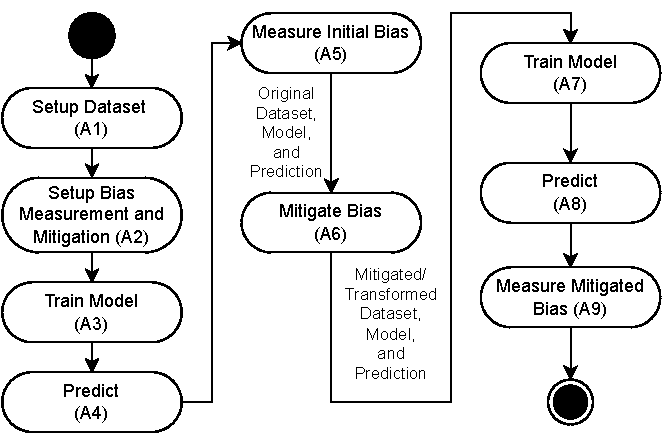
\includegraphics[width=\linewidth]{figures/workflow}
	%%	\caption{The workflow of bias mitigation commonly performed using the toolkits in Section \ref{sec:toolkits}.}
	%%	\label{fig:workflow}
	%%\end{figure}
	%
	
	\textbf{Set Up Datasets (T01)}. Bias mitigation commonly starts with \textit{datasets} setup. In this task, users define the \textit{source} of every dataset which is commonly a \textit{CSV file}. They also determine which attribute is the \textit{predicted attribute}, including the \textit{favourable class} in the attribute, and the \textit{sensitive attributes} as well as their \textit{privileged} and \textit{unprivileged classes}. The datasets can also be loaded from the \textit{built-in datasets} provided by certain toolkits. 
	The \textit{training}, \textit{validation}, and \textit{test datasets} are also set here, whether they are all come from different datasets or the same dataset but is \textit{split} in different ratios. They also select the \textit{bias metrics} and \textit{mitigation algorithms} that will be applied to datasets, \textit{models}, and \textit{prediction}. 
	
	\textbf{Measure Original Biases Prior Prediction (T02)}. In this task, users measure the \textit{original biases} of the datasets in different metrics, such as accuracy, mean difference, etc. The results are later used as benchmarks when compared with the measurement results after prediction (T04) or bias mitigation (T06).  
	
	\textbf{Train and Predict (T03)}. This task \textit{trains} \textit{models} commonly using certain \textit{classifiers}/\textit{classification algorithms} on the train datasets defined in Task T01. If required, the training can extend to \textit{validation} to tune hyper-parameters in order to obtain the best \textit{parameters} for the models. After that, users use the models to \textit{predict} on the test datasets defined in Task T01. This task can be skipped if a prediction is not required. For example, we want to measure and mitigate biases only in the original datasets (pre-processing).
	
	\textbf{Measure Original Biases Post Prediction (T04)}. In this task, users measure the original accuracies and biases after performing the prediction in Task T03. The results are used as benchmarks later when comparing them against biases after bias mitigation. This action is skipped if prediction or Task T03 is not performed.
	
	\textbf{Mitigate Bias (T05)}. In this task, users choose the type of debiasing algorithms -- pre-processing, in-processing, or post-processing -- they want to apply. \textit{Validation} can also be performed if hyper-parameter tuning is required to obtain the best parameters for the debiasing algorithms.
	%\begin{itemize}
	%	\item[a.] \textbf{Pre-processing}. Before model training and prediction, users apply debiasing algorithms to the (copies of) original datasets.
	%	\item[b.] \textbf{In-processing}. Users apply debiasing algorithms to regulate the training process to become fairer for protected groups when predicting.
	%	\item[c.] \textbf{Post-processing}. Users apply debiasing algorithms to the prediction results to make them fairer for protected groups. 
	%\end{itemize}
	
	\textbf{Measure Biases After Debiasing (T06)}. In this task, users measure accuracies and biases after applying debiasing algorithms in Task T05 using the test datasets. 
	
	\textbf{Conclude (T07)}. In this task, the biases after debiasing are compared against the original biases obtained in Tasks T02 and T04. Users then analyse the results to find the best combinations of datasets, classifiers, and debiasing algorithms with biases and accuracy that fit their purposes. The comparisons can be presented in numbers, tables, and charts to facilitate users to analyse the effects of the datasets, classifiers, and debiasing algorithms. 
	
	\subsection{Metamodel}
	\label{sec:metamodel}
	
	\begin{figure}
		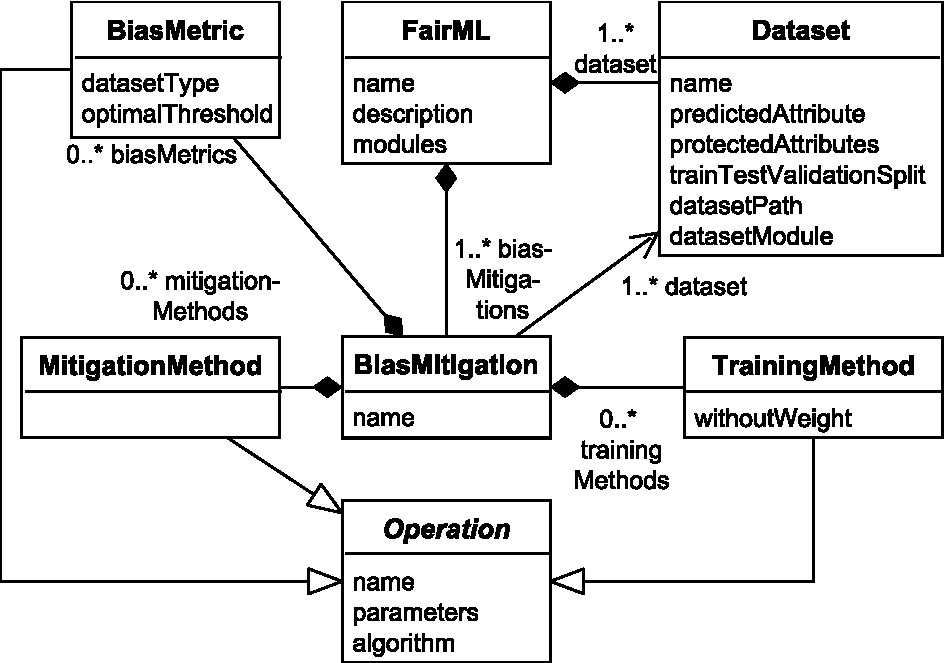
\includegraphics[width=\linewidth]{figures/metamodel}
		\caption{The Metamodel of FairML.}
		\label{fig:metamodel}
	\end{figure}
	
	The identified important constructs are then translated into FairML's metamodel so that users can express them when defining their bias mitigation. Figure \ref{fig:metamodel} shows a simplified version of the metamodel. The \texttt{FairML} class represents a project of bias mitigation in machine learning. It can contain one or more datasets and bias mitigations. 
	
	The \texttt{Dataset} class defines the datasets. In the class, we specify a dataset's name, predicted attribute, protected attributes, the split ratio between train, test, and validation, and the path of its CSV file. We can also use a dataset from the built-in IBM AI Fairness 360's datasets by specifying its Python module in the \texttt{datasetModule} attribute.
	
	The \texttt{BiasMitigation} class specifies the bias mitigations to be executed in the FairML project. The \textit{name} attribute is used as the identifier of bias mitigations. The class contains three other significant classes: \texttt{TrainingMethod}, \texttt{MitigationMethod}, and \texttt{BiasMetric}. All of them are derived from the \texttt{\textit{Operation}} abstract class since they can be executed, have parameters, and return certain results. The attributes \textit{name} and \textit{parameters} are used as the identifiers and to define the parameters of operations respectively. The \texttt{algorithm} attribute of the \texttt{Operation} class defines the selected algorithms executed by each deriving class. The \texttt{TrainingMethod} class is responsible to define the classifiers for training and prediction, while the \texttt{MitigationMethod} class specifies the debiasing algorithms for bias mitigation. \texttt{BiasMetric} class determines the metrics to be used to measure fairness. 
	
	
	\subsection{Generation}
	\label{sec:generation}
	
	Figure \ref{fig:transformation} depicts the the transformation applied by FairML to transform a bias mitigation model into Python and Jupyter Notebook files. Users define their bias mitigation models in Flexmi\footnote{\url{https://www.eclipse.org/epsilon/doc/flexmi}} \cite{dimitris2016flexmi}. The model then is transformed by Epsilon Generation Language (EGL) \cite{rose2008egl} engine into Python code. The transformation follows the FairML's EGX/EGL\footnote{\url{https://www.eclipse.org/epsilon/doc/egl/}} rules and conforms to the defined FairML's metamodel in Ecore \cite{steinberg2009emf}. The generated Python files are then transformed into Jupyter notebook files using P2J\footnote{\url{https://pypi.org/project/p2j/}} engine.
	
	\begin{figure}
		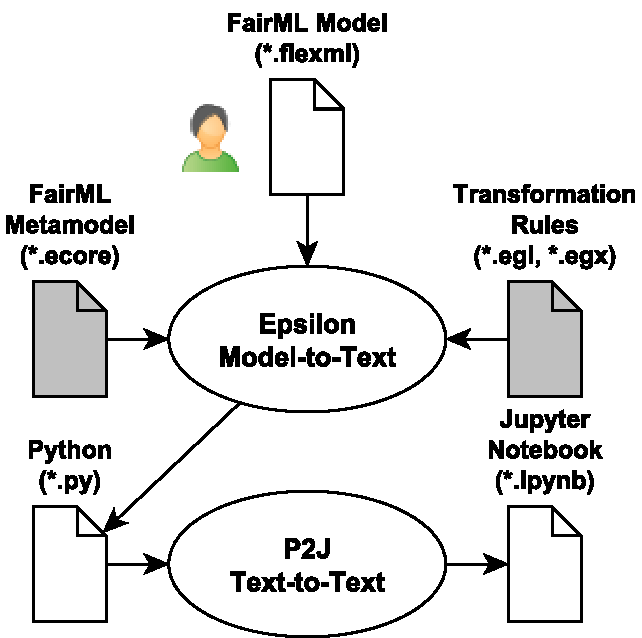
\includegraphics[width=\linewidth]{figures/transformation}
		\caption{Model-to-text transformation in fairML.}
		\label{fig:transformation}
	\end{figure}
	
	
	
	\subsection{FairML Example}
	\label{sec:fairml_example}
	Listing \ref{lst:fairml_model} shows a FairML model, that conforms to the metamodel in Figure\ref{fig:metamodel}, expressed in YAML. The model is the FairML version of 
	IBM AI Fairness 360's Exponentiated Gradient Reduction\footnote{\url{https://github.com/Trusted-AI/AIF360/blob/master/examples/demo_exponentiated_gradient_reduction.ipynb.}} demo. The original example has 93 lines, excluding commented and empty lines, almost three times the lines of code expressed in the listing.
	
	The model has a name and description, \texttt{Demo} and \texttt{Debiasing using EGR} respectively, as well as adding some Python modules to be used in its components (lines 1-6). The \texttt{modules} feature is for adding additional modules that are not automatically loaded in the generated code. In the Listing, we add \texttt{load\_preproc\_data\_adult} module that is used in the \texttt{dataset} component.
	
	The model has one dataset and one bias mitigation. The dataset is named \texttt{Adult} and is loaded from a preprocessed adult dataset provided by IBM AI Fairness 360 using \texttt{load\_preproc\_data\_adult} function. We also set \texttt{sex} as its protected attribute and split it to train test, and validation with ratios 7:3:0 (lines 8-13). 
	
	Lines 16-36 defines the definition of the bias mitigation executed in the \texttt{Demo} model. The bias mitigation is named \texttt{Exponentiated Gradient Reduction} and use the \texttt{Adult} dataset defined at lines 9-13 as its \texttt{dataset}. 
	
	The bias mitigation uses three different metrics to analyse the trade-off between accuracy and fairness (mean difference, average odds difference) (lines 29-34) when the prediction uses a Logistic Regression classifier only without debiasing (lines 20-22) and when the prediction is debiased using Exponentiated Gradient Reduction (lines 24-27). The former only uses one parameter; \texttt{'lbfgs'} is set as the \texttt{solver}, while the latter has three parameters; the same classifier is used as the \texttt{estimator}, \texttt{'EqualizedOdds'} is used as the \texttt{constraint}, and the protected attributes are not dropped.
	
\begin{lstlisting}[firstnumber=1,style=yaml,caption={Bias mitigation using  Demo Exponentiated Gradient Reduction  expressed in YAML.},label=lst:fairml_model]
?nsuri: fairml
fairml:
- name: Demo
- description: Debiasing using EGR
- modules: 
from aif360.algorithms.preprocessing.optim_preproc_helpers.data_preproc_functions import load_preproc_data_adult

# set the dataset
- dataset:
- name: Adult
- datasetModule: load_preproc_data_adult
- protectedAttributes: sex
- trainTestValidationSplit: 7, 3

# define the bias mitigation
- biasMitigation:
- name: Exponentiated Gradient Reduction  
- dataset: Adult

- trainingMethod:
- algorithm: LogisticRegression
- parameters: solver='lbfgs'

- mitigationMethod:
- algorithm: ExponentiatedGradientReduction
- parameters: 
estimator=LogisticRegression(solver='lbfgs'), constraints='EqualizedOdds', drop_prot_attr=False

- biasMetric:
- name: accuracy
- biasMetric:
- name: mean_difference
- biasMetric:
- name: average_odds_difference
\end{lstlisting}

	\subsection{Wizard}
	\label{sec:wizard}
	There are many available debiasing algorithms and bias metrics that users can select to mitigate biases in machine learning. Some of them are better than others in a certain context. FairML has a wizard feature that assists users in selecting the most appropriate debiasing algorithms and bias metrics based on their answers to the wizard's questions. Some of the questions are listed in Listing  \ref{lst:wizard_questions}. The wizard follows the guidances suggested by \cite{mahoney2020ai}, IBM AI Fairness 360\footnote{\url{https://aif360.mybluemix.net/resources\#guidance}}, and Aequitas\footnote{\url{http://aequitas.dssg.io/static/images/metrictree.png}}. After completing the wizard, FairML automatically generates a FairML model (*.flexmi) and its Python and Jupyter notebook files.
	
\begin{lstlisting}[firstnumber=1,style=yaml,caption={Some the questions asked in the FairML's wizard to assist users to select the best debiasing algorithms and bias metrics.},label=lst:wizard_questions]
...
---- Mitigation Algorithm ----
# 1. Pre-processing
Apply bias mitigation in pre-processing (default: true): 
The weights of the dataset are modifiable (default: true): 
The bias mitigation allows latent space (default: false): 
...
...
---- Bias Metric ----
Measure group fairness (default: true): 
Measure individual fairness (default: false): 
Use single metrics for both individuals and groups (default: false): 
Measure equal fairness (default: false):
... 
\end{lstlisting}
	
	\subsection{Generated Files}
	\label{sec:generated_files}
	Based on the model defined in Listing \ref{lst:fairml_model}, FairML generates a Jupyter notebook file containing the code that performs the bias mitigation, an explanation of the bias measured, and references to the selected classifiers and debiasing algorithms to help users understand the applied bias mitigation and metrics measured. It also contains a table and chart that compares the bias metrics measured by different datasets, classifiers, and debiasing algorithms to help users select the best combinations that fit their contexts. 
	
	As an example, Figure \ref{fig:table-output} shows the summary table of the bias measurements produced by Listing \ref{lst:fairml_model}. There are three combinations of prediction. In the first combination, we only measure the Mean Difference, a.k.a. Statistical Parity Difference, in the original dataset. After performing prediction using Logistic Regression, the second combination measures some metrics without any bias mitigation. The table shows the mean difference is slightly worsened to -0.206, moving away from 0, advantaging the privileged group (negative sign). After applying the Exponentiated Gradient Reduction as the debiasing algorithm, the prediction accuracy is slightly reduced to 0.79 but with significant improvement in fairness; the Mean Difference and Average Odds Difference are closer to zero than their values prior the bias mitigation.
	
	
	\begin{figure*}
		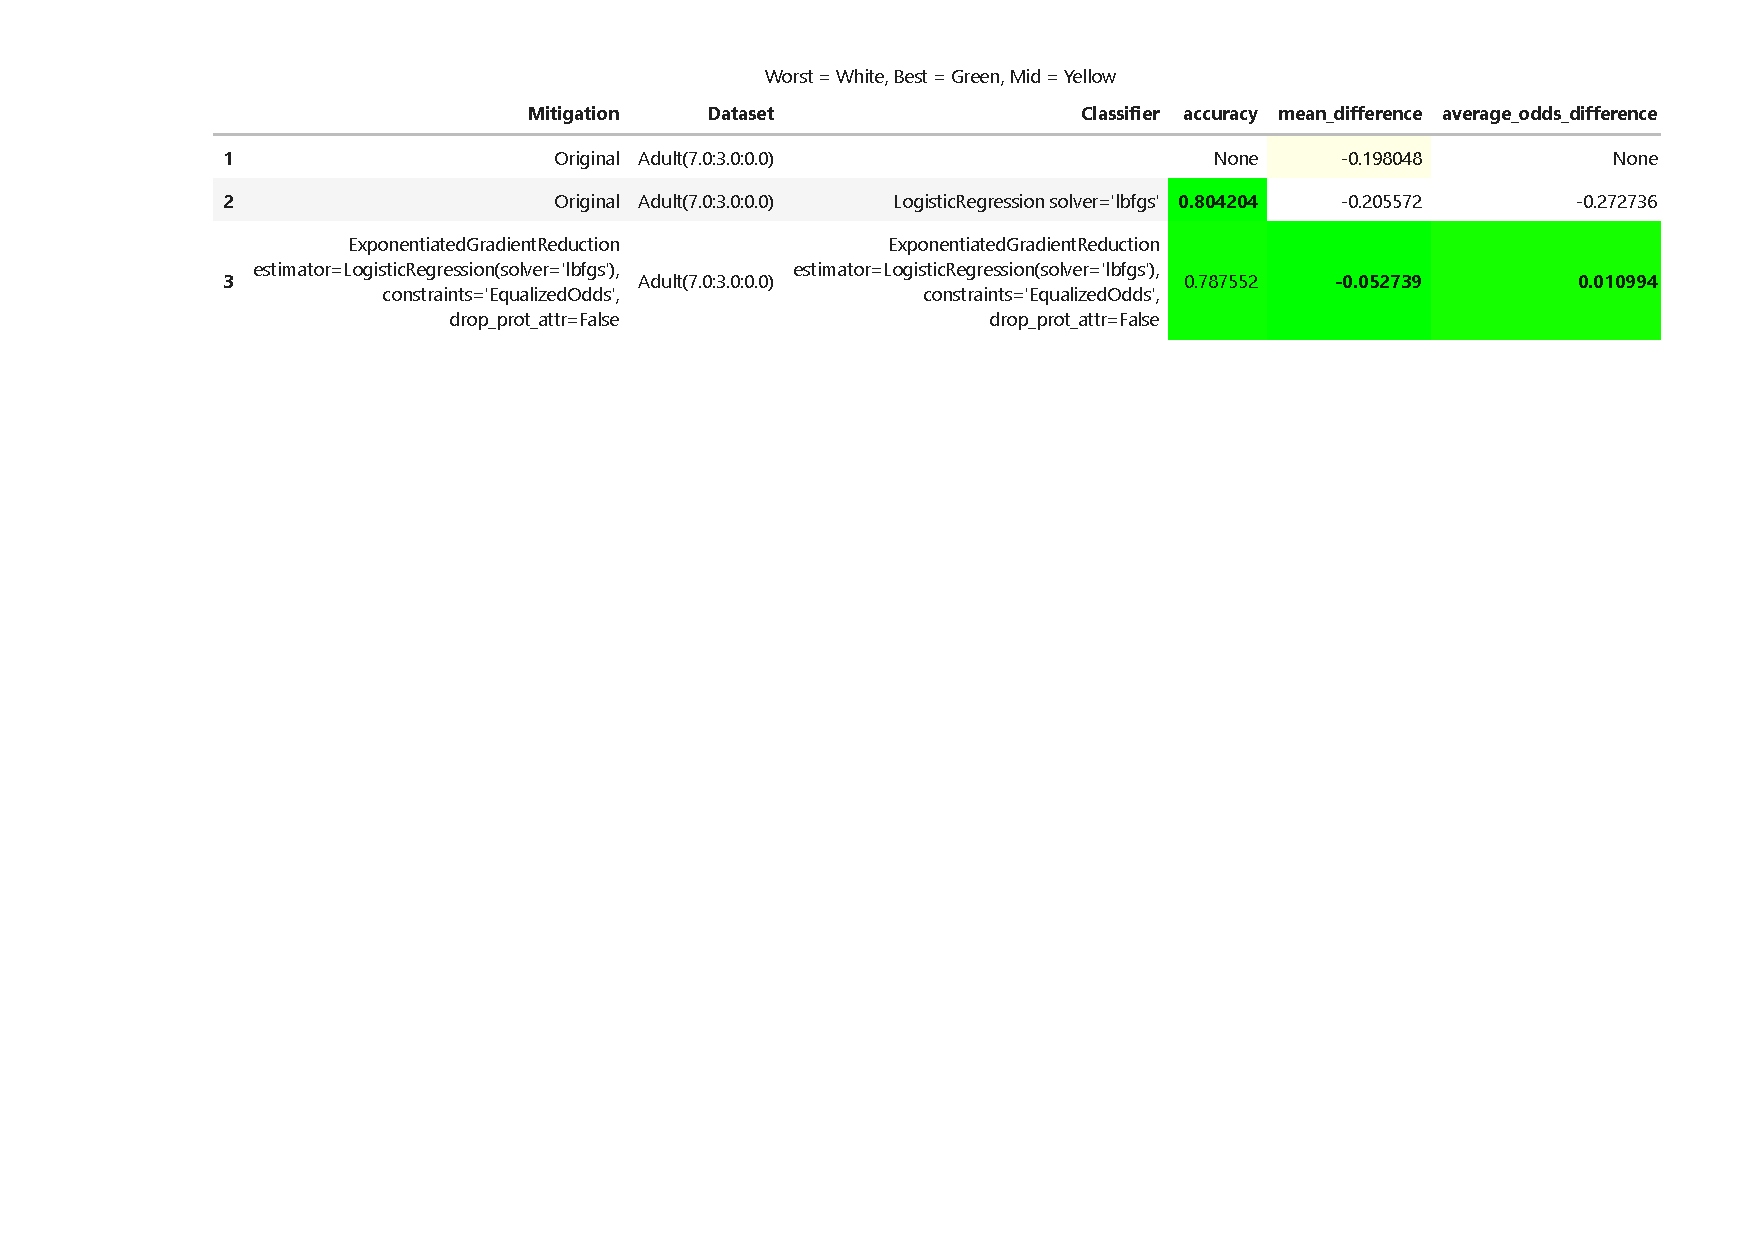
\includegraphics[width=\linewidth]{figures/table-output}
		\caption{The summary table displayed in the generated Juypter notebook file based on the model defined in Listing \ref{lst:fairml_model}.}
		\label{fig:table-output}
	\end{figure*}
	
	
	\newcolumntype{L}[1]{>{\raggedright\arraybackslash}p{#1}}
	\newcolumntype{C}[1]{>{\centering\arraybackslash}p{#1}}
	\newcolumntype{R}[1]{>{\raggedleft\arraybackslash}p{#1}}
	\begin{table*}[]
		\caption{Part 1 of 2 -- IBM AI Fairness 360 examples and the numbers of unique datasets, classifiers, de-biasing algorithms, bias metrics, and measurement values in each example.}
		\label{tab:expressiveness1}
		\begin{tabular}{ p{1em} L{10em} R{4em} R{8em} R{9em} R{12em} R{2.5em} }
			\hline
			\multicolumn{1}{c}{\textbf{Code}} &
			\multicolumn{1}{c}{\textbf{\begin{tabular}[c]{@{}c@{}}Example/File Name\\ (*.ipynb)\end{tabular}}} &
			\multicolumn{1}{c}{\textbf{Datasets}} &
			\multicolumn{1}{c}{\textbf{Classifiers}} &
			\multicolumn{1}{c}{\textbf{\begin{tabular}[c]{@{}c@{}}Debiasing\\ Algorithms\end{tabular}}} &
			\multicolumn{1}{c}{\textbf{\begin{tabular}[c]{@{}c@{}}Bias\\Metrics\end{tabular}}} &
			\multicolumn{1}{c}{\textbf{\begin{tabular}[c]{@{}c@{}}Mea-\\sure-\\ments\end{tabular}}} \\ \hline
			E01 &
			Demo Adversarial Debiasing &
			Adult &
			N/A &
			Adversarial debiasing &
			Accuracy, Balanced accuracy, Disparate impact, Average odds, Statistical parity, Equal opportunity, Theil index &
			28 \\
			E02 &
			Demo Callibrated Eq Odd Postprocessing &
			Adult, German, Compas &
			Logistic regression &
			Calibrated eq odds postprocessing &
			Mean difference, False positive rate, False negative rate, Balanced accuracy, Equal opportunity &
			13 \\
			E03 &
			Demo Disparate Impact Remover &
			Adult &
			Logistic regression &
			Disparate impact remover &
			Disparate impact &
			11 \\
			E04 &
			Demo Exponentiated Gradient Reduction &
			Adult &
			Logistic regression &
			Exponentiated gradient reduction &
			Accuracy, Mean difference, Average odds &
			8 \\
			
			E05 &
			Demo LFR &
			Adult &
			Logistic regression &
			Learning fair representation &
			Balanced accuracy, Mean difference, Disparate impact &
			5 \\
			E06 &
			Demo Meta Classifier &
			Adult &
			N/A &
			Meta fair classifier &
			Accuracy, Balanced accuracy, Disparate impact, False discovery rate &
			13 \\
			E07 &
			Demo Optim Preproc Adult &
			Adult &
			N/A &
			Optimized preprocessing &
			Mean difference &
			2 \\
			E08 &
			Demo Reject Option Classification &
			Adult, German, Compas &
			Logistic Regression &
			Reject option classification &
			Balanced accuracy, Disparate impact, Average odds, Statistical parity, Equal opportunity, Theil index &
			26 \\
			E09 &
			Demo Reweighing Preproc &
			Adult, German, Compas &
			Logistic Regression &
			Reweighing &
			Balanced accuracy, Disparate impact, Average odds,. Statistical parity, Equal opportunity, Theil index &
			16 \\
			E10 &
			Demo Short Gerryfair Test &
			Adult &
			Linear Regression, Linear SVR, Decision Tree, Kernel Ridge &
			Gerryfair &
			Gamma disparity &
			13 \\
			E11 &
			Tutorial Credit Scoring &
			German &
			N/A &
			Reweighing &
			Mean difference &
			2 \\
			E12 &
			Tutorial Medical Expenditure &
			MEPS-Dataset19, MEPSDataset20, MEPSDataset21 &
			Random Forest, Logistic Regression &
			Reweighing, Prejudice remover &
			Balanced accuracy, Disparate impact, Average odds, Statistical parity, Equal opportunity, Theil index &
			90 \\
			\hline
		\end{tabular}
	\end{table*}
	
	%\begin{table*}[]
	%	\caption{Part 2 of 2 -- IBM AI Fairness 360 examples and the numbers of unique datasets, classifiers, de-biasing algorithms, bias metrics, and measurement values in each example.}
	%	\label{tab:expressiveness2}
	%	\begin{tabular}{ p{1em} L{10em} R{4em} R{8em} R{9em} R{12em} R{2.5em} }
		%		\hline
		%		\multicolumn{1}{c}{\textbf{Code}} &
		%		\multicolumn{1}{c}{\textbf{\begin{tabular}[c]{@{}c@{}}Example/File Name\\ (*.ipynb)\end{tabular}}} &
		%		\multicolumn{1}{c}{\textbf{Datasets}} &
		%		\multicolumn{1}{c}{\textbf{Classifiers}} &
		%		\multicolumn{1}{c}{\textbf{\begin{tabular}[c]{@{}c@{}}Debiasing\\ Algorithms\end{tabular}}} &
		%		\multicolumn{1}{c}{\textbf{\begin{tabular}[c]{@{}c@{}}Bias\\Metrics\end{tabular}}} &
		%		\multicolumn{1}{c}{\textbf{\begin{tabular}[c]{@{}c@{}}Mea-\\sure-\\ments\end{tabular}}} \\ \hline
		%		
		%		E05 &
		%		Demo Gerryfair &
		%		Adult &
		%		Linear Regression, Linear SVR, Decision Tree, Kernel Ridge &
		%		Gerryfair &
		%		Gamma disparity &
		%		31 \\
		%		E07 &
		%		Demo Lime &
		%		Adult &
		%		Logistic regression, Random forest &
		%		Reweighing &
		%		Accuracy, Balanced accuracy, Disparate impact, Average odds &
		%		6 \\
		%		E08 &
		%		Demo MDSS Classifier Metric &
		%		Compas &
		%		Logistic regression &
		%		Meta fair classifier &
		%		Mean difference, MDSS bias score &
		%		7 \\
		%		E10 &
		%		Demo Optim Data Preproc &
		%		Adult, German, Compas &
		%		Logistic regression &
		%		Optimized preprocessing &
		%		Balanced accuracy, Disparate impact, Average odds, Statistical parity &
		%		9 \\
		%	
		%		E17 &
		%		Demo Exponentiated Gradient Reduction Sklearn &
		%		Adult &
		%		Logistic Regression &
		%		Grid search reduction &
		%		\begin{tabular}[c]{@{}r@{}}Average odds\\ Accuracy\end{tabular} &
		%		7 \\
		%		E18 &
		%		Demo Grid Search Reduction Classification Sklearn &
		%		Adult &
		%		Logistic Regression &
		%		Grid search reduction &
		%		Average odds, Accuracy &
		%		4 \\
		%		E19 &
		%		Demo Grid Search Reduction Regression Sklearn &
		%		Lawschool GPA &
		%		Linear Regression &
		%		Grid search reduction &
		%		Mean absolute error &
		%		7 \\
		%		E20 &
		%		Demo MDSS Classifier Metric Sklearn &
		%		Compas &
		%		Logistic Regression &
		%		N/A &
		%		MDSS bias score &
		%		4 \\
		%		E21 &
		%		Demo New Features &
		%		Adult &
		%		Logistic Regression &
		%		Reweighing meta, Adversarial debiasing, Callibrated equalized odd &
		%		Disparate impact, Average odds, Mean difference, Accuracy &
		%		6 \\ \hline
		%	\end{tabular}
	%\end{table*}
	
	\begin{table*}[]
		\caption{Comparison of numbers of lines of code between original examples (Original LoC), FairML models (Model LoC), and generated code (Generated LoC) as well as the generation time of FairML and the execution time of the original examples and generated code (seconds). See Table \ref{tab:expressiveness1} 
			%	and \ref{tab:expressiveness2} 
			for the titles of the examples on the second column.}
		\label{tab:evaluation}
		\begin{tabular}{crrrrrrrrrr}
			\hline
			\textbf{Code} &
			\multicolumn{1}{c}{\textbf{\begin{tabular}[c]{@{}c@{}}Ori\\ LoC\end{tabular}}} &
			\multicolumn{1}{c}{\textbf{\begin{tabular}[c]{@{}c@{}}Model\\ LoC\end{tabular}}} &
			\multicolumn{1}{c}{\textbf{\begin{tabular}[c]{@{}c@{}}Gen\\ LoC\end{tabular}}} &
			\multicolumn{1}{c}{\textbf{\begin{tabular}[c]{@{}c@{}}Model  LoC/\\ Ori  LoC\end{tabular}}} &
			\multicolumn{1}{c}{\textbf{\begin{tabular}[c]{@{}c@{}}Gen LoC/\\ Model LoC\end{tabular}}} &
			\multicolumn{1}{c}{\textbf{\begin{tabular}[c]{@{}c@{}}Gen LoC/\\ Ori LoC\end{tabular}}} &
			\multicolumn{1}{c}{\textbf{\begin{tabular}[c]{@{}c@{}}Generation\\ Time\end{tabular}}} &
			\multicolumn{1}{c}{\textbf{\begin{tabular}[c]{@{}c@{}}Original\\ Exec Time\end{tabular}}} &
			\multicolumn{1}{c}{\textbf{\begin{tabular}[c]{@{}c@{}}Generated\\ Exec Time\end{tabular}}} &
			\multicolumn{1}{c}{\textbf{\begin{tabular}[c]{@{}c@{}}Gen/Ori\\ Time\end{tabular}}} \\ \hline
			E01 & 133 & 41 & 128 & 0.31 & 3.12 & 0.96 & 0.17 & 96.21 & 102.98 & 1.07 \\
			E02 & 257 & 37 & 170 & 0.14 & 4.59 & 0.66 & 0.17 & 7.93 & 2.33 & 0.29 \\
			E03 & 50 & 50 & 375 & 1.00 & 7.50 & 7.50 & 0.19 & 20.99 & 20.23 & 0.96 \\
			E04 & 93 & 33 & 118 & 0.35 & 3.58 & 1.27 & 0.17 & 29.93 & 30.21 & 1.01 \\
			E05 & 103 & 37 & 91 & 0.36 & 2.46 & 0.88 & 0.16 & 218.05 & 207.78 & 0.95 \\
			E06 & 95 & 67 & 345 & 0.71 & 5.15 & 3.63 & 0.20 & 12.99 & 14.67 & 1.13 \\
			E07 & 35 & 30 & 86 & 0.86 & 2.87 & 2.46 & 0.14 & 8.04 & 15.52 & 1.93 \\
			E08 & 143 & 61 & 146 & 0.43 & 2.39 & 1.02 & 0.16 & 12.97 & 15.57 & 1.20 \\
			E09 & 212 & 59 & 138 & 0.28 & 2.34 & 0.65 & 0.17 & 1.46 & 4.63 & 3.17 \\
			E10 & 52 & 55 & 176 & 1.06 & 3.20 & 3.38 & 0.17 & 3.39 & 3.88 & 1.14 \\
			E11 & 30 & 25 & 85 & 0.83 & 3.40 & 2.83 & 0.17 & 0.02 & 0.08 & 4.59 \\
			E12 & 356 & 90 & 644 & 0.25 & 7.16 & 1.81 & 0.22 & 34.90 & 54.25 & 1.55 \\
			%		E13 & 54  &    &     &      &      &      &       &        &        &      \\
			%		E14 & 54  &    &     &      &      &      &       &        &        &      \\
			%		E15 & 54  &    &     &      &      &      &       &        &        &      \\
			%		E16 & 54  &    &     &      &      &      &       &        &        &      \\
			%		E17 & 54  &    &     &      &      &      &       &        &        &      \\
			%		E18 & 52  &    &     &      &      &      &       &        &        &      \\
			%		E19 & 64  &    &     &      &      &      &       &        &        &      \\
			%		E20 & 66  &    &     &      &      &      &       &        &        &      \\
			%		E21 & 82  &    &     &      &      &      &       &        &        &      \\ 
			\hline
		\end{tabular}
	\end{table*}
	
	\section{Evaluation}
	\label{sec:evaluation}
	In this research, we also evaluated the expressiveness, correctness, productivity, and execution time of FairML. In the expressiveness evaluation, we aimed to answer this question, 
	``\textit{Can FairML express the use cases of bias mitigation in the real-world?}''. For that, we used the examples provided by IBM Fairness AI 360 as the baseline to justify the expressiveness of FairML. 
	the toolkit comes with some examples (Table \ref{tab:expressiveness1})
	% and \ref{tab:expressiveness2})
	that demonstrate 
	the use-cases of the toolkit in the real-world context. 
	We used the 12 examples that come in version 3.0 of the toolkit.
	%Among 22 examples in version 3.0, we only used 21 of them, 
	%since the one that we excluded only explains the use of a class dedicated to yield bias metric explanation in JSON format. 
	We also count the numbers of bias metrics, debiasing algorithms, classifiers, datasets, and measurement values in each example to reveal its complexity. 
	
	We compared the bias metric values measured (measurement values) in the original examples with the values measured in the generated code to evaluate the correctness of FairML's generated code. Both should produce equal or similar values, up to 10\% tolerance, when randomness is required.  
	
	In the productivity evaluation, 
	we compared the ratio of the written vs. generated code of FairML vs.
	Code in the examples. 
	While this metric does not always guarantee productivity due to many factors, 
	the number of lines written by users is significantly reduced. In the measurement, \textit{markdown}, whitespace, and commented lines were not counted.
	
	We also measured the execution time of FairML. First, we measured the \textit{generation time} -- the time that FairML takes to generate the target code. Second, we compared the time taken by the generated target code against the example code to complete their operations (\textit{generated execution time} vs. \textit{original execution time}). The evaluation was performed on a machine with Windows 10 64-bit operating system, 11th Gen Intel(R) Core(TM) i9-11900H @ 2.50GHz 8-core processors, 32.0 GB RAM DDR4, OpenJDK Runtime Environment 18.9 (build 11.0.14.1+1), and Python 3.9.7.
	
	\section{Results and Discussion}
	\label{sec:result_and_discussion}
	In this section, we present and discuss the results of our FairML evaluation.
	
	\subsection{Expressiveness and Correctness}
	\label{sec:expressiveness_and_correctness}
	Based on our evaluation, FairML was able to reproduce all the scenarios in all the 12 examples in Table \ref{tab:expressiveness1}.
	%and \ref{tab:expressiveness2}.
	In total, all the scenarios covered six unique datasets 
	(Adult, German, Compas, MEPSDataset19, MEPSDataset20, MEPSDataset21)
	%(Adult, German, Compas, Lawschool GPA, MEPSDataset19, MEPSDataset20, MEPSDataset21), 
	Six classifiers (Logistic Regression, Linear Regression, Linear SVR, Decision Tree, Kernel Ridge, Random Forest), 
	11 bias mitigation algorithms 
	(Adversarial Debiasing, Calibrated Equalising Odds, Disparate Impact Remover, Exponentiated Gradient Reduction, Gerryfair, Learning Fair Representation, Reweighing, Meta Fair Classification, Optimized Preprocessing, Reject Option Classification, Prejudice Remover), 
	%(Adversarial Debiasing, Calibrated Equalising Odds, Disparate Impact Remover, Exponentiated Gradient Reduction, Gerryfair, Learning Fair Representation, Reweighing, Meta Fair Classification, Optimized Preprocessing, Reject Option Classification, Prejudice Remover, Grid Search Reduction, Reweighing Meta), 
	and 
	13 bias metrics 
	(Accuracy, Balanced Accuracy, Mean Difference, Statistical Parity Difference, Disparate Impact, Equal Opportunity Difference, Theil Index, Gamma Disparity, Average Odds Difference, Mean Absolute Error, False Positive Rate, False Negative Rate, False Discovery Rate). 
	%(Accuracy, Balanced Accuracy, Mean Difference a.k.a. Statistical Parity Difference, Disparate Impact, Equal Opportunity Difference, Theil Index, Gamma Disparity, Average Odds Difference, Mean Absolute Error, MDSS Bias Score, False Positive Rate, False Negative Rate, False Discovery Rate, Rrror Rate, Mean Absolute Error). 
	In addition, FairML also supports loading data from external CSV files. These allow users to express their bias mitigation strategies in different combinations of datasets, classifiers, debiasing algorithms, and bias metrics.
	
	Regarding correctness, due to the randomness in machine learning processes, not all values produced by the generated code are precisely equal to their respective values in the examples. Thus, we use $\pm$ 0.1 tolerance for the differences to ensure that the generated code's values are almost equal to their respective ones.
	
	%From all $N$ measurement values in Tables \ref{tab:expressiveness1} and \ref{tab:expressiveness2}, equal values comprise $N1$ values, while the tolerated values cover only $N2$ values.  
	
	\subsection{Productivity}
	\label{sec:productivity}
	
	Table \ref{tab:evaluation} shows a comparison of the numbers of lines of code (LoC) between the original examples, FairML models, and generated code. It shows that \textsf{Model LoC}/\textsf{Original LoC} are equal to or less than 1, indicating that users would write less code to produce the same results as in the examples (see Section \ref{sec:expressiveness_and_correctness} for correctness). Moreover, the efficiency also gets higher as the number of original LoC increases. This can been seen at the examples \textsf{E15} and \textsf{E16}, where LoC goes up from 30 to 356, that the efficiency is also increased with users only need to write from 83\% to 25\% of the LoC in their respective original examples.
	
	We do expect that FairML generates more LoC than the original examples as they contain features that are not included in the original examples, such as (1) the code for explaining the classifiers, bias mitigation algorithms, and bias metrics being used, as well as (2) the code for displaying summary tables and charts. 
	
	%We admit that there are also generated lines of code that are not always necessary for every scenario but always exist in the code -- this also increases the number of generated LoC.For example,   
	
	
	
	\subsection{Execution Time}
	\label{sec:execution_time}
	
	Table \ref{tab:evaluation} shows the duration -- generation time -- taken by FairML to produce generated code, 
	and the performance of the generated code on execution time against the original examples (in seconds). 
	In the generation time, 
	FairML can generate every generated-code version of the original examples in less that 0.2 seconds, 
	and it can achieve the rate 2,798 lines/second based on the example E16 
	(554 lines/0.198 seconds, Table \ref{tab:evaluation}). 
	
	In general, the execution time of the generated code takes more time than the original examples. 
	We do anticipate this as the generated-code versions have more features, having more lines of code,
	as stated in Section \ref{sec:productivity}. 
	
	\subsection{Threats to Validity}
	\label{sec:threats_to_validity}
	While we have tested FairML with the examples of IBM AI Fairness 360, we have not performed user evaluation due to limited resources to obtain feedback from experienced users in the field. Also, there is a chance that the examples do not reflect bias mitigation in the real world. These threats have been identified by \cite{lee2021landscape} as the adoption of fairness toolkits is still not a common practice.
	
	\section{Lessons Learned}
	\label{sec:lessons_learned}
	As the adoption of fairness toolkits is still not a common practice \cite{lee2021landscape}, it was challenging for us to perform domain analysis and user evaluation to obtain feedback from the experienced users in the field. As a solution, we opted for document analysis as documents contain information to understand the objects of interest \cite{bowen2009document}. We analysed the code repository and documentation of IBM AI Fairness 360, as they can reflect the bias mitigation in practice to understand its uses and implementation in mitigating bias in machine learning. Through the documentation and code repository of the toolkit, we identified the important constructs and workflows of bias mitigation in machine learning and used them to construct FairML. We also use the examples provided by the toolkit as the benchmark for the correctness and performance evaluation of the generated bias mitigation code. 
	
	The other challenge is in generating Jupyter notebook (IPYNB) files. We want to support users so that they can add their code into the files or modify existing code without being overridden when the code generation is re-executed. Initially, we aimed to add protected regions into the IPYNB files. However, since an IPYNB file is a JSON file, it does not support \textit{commenting}. The inability invalidated our approach that used EGL engine \cite{rose2008egl} for adding protected regions as the engine relies on commenting characters to mark protected areas. As a solution, we use Python files as the intermediate generated files, as Python code supports commenting, and a third-party P2J engine to covert the Python files to Jupyter notebook files. However, this solution is imperfect as users can only modify the Python files if they want their own code or modify existing code to be preserved.
	
	\section{Related Work}
	\label{sec:related_work}
	
	Some toolkits have been developed to measure biases in machine learning. 
	Another FairML, a toolbox developed by \cite{adebayo2016fairml}, audits the fairness of a predictive model by calculating the relative effects of its different inputs on its predictions by leveraging four input ranking algorithms and model compression. 
	FairTest \cite{tramer2017fairtest} calculates the associations between sensitive attributes and predicted labels to check biases in a dataset. It also provides a methodology to identify the input space's regions where an algorithm might produce unusual high rates of errors.
	Themis \cite{galhotra2017themis}, a bias toolbox, allows automatic generation of tests to measure discrimination in the decisions of a predictive system.
	Fairness Measures \cite{zehlike2017fairness} supports the measurement of different bias metrics, such as disparate impact, average odds ratio, and mean difference. 
	Aequitas \cite{saleiro2019aequitas} is an auditing toolkit that measures fairness in different metrics. It also provides a decision tree to guide users in choosing the most appropriate metrics for a particular situation. 
	
	Some other toolkits are also able to mitigate biases, not only for measuring fairness. They are ThemisML \cite{bantilan2018themis}, Fairness Comparison \cite{friedler2019fairness}, Aequitas\cite{saleiro2019aequitas}, Google What-If\cite{googlewhatif2020}, Scikit-fairnet/scikit-lego \cite{scikitfairness2022,scikitlego2022}, Fairlearn\cite{bird2020fairlearn}, and IBM AI Fairness 360 \cite{bellamy2018ai}.
	
	Rapidminer \cite{hofmann2016rapidminer}, Knime \cite{berthold2008knime}, and Orange \cite{demsar2013orange} are the platforms that use low-code, model-based approaches to allow users to visually program machine learning pipelines by assembling component-based procedures. They support data exploration, transformation, visualisation, and different algorithms for machine learning and data mining. Moreover, all of them are extensible, which means users can add new modules or scripts. However, as far as we are aware, there are no built-in modules for measuring and mitigating biases. 
	
	The closest existing work to FairML is Arbiter \cite{zucker2020arbiter}, a domain specific-language designed for ethical machine learning. It is an SQL-like declarative language to define how to train machine learning models with four components to describe its ethical practices: transparency, fairness, accountability, and reproducibility. Unfortunately, the implementation is limited only to a particular metric and classifier\footnote{\url{https://github.com/julian-zucker/arbiter}}.
	
	\section{Conclusions and Future Work}
	\label{sec:conclusions_and_future_work}
	This paper presents FairML, a toolkit that implements a model-based approach to automate bias mitigation. Using FairML, users can generate bias mitigation code by writing fewer lines in YAML than writing the code in Python, a general programming language.
	The generated code produces the same bias metric values as measured in the original examples in terms of correctness.
	
	As the development of FairML is still in the early stage, 
	there is much room for improvement in future work. For example, the number of lines of code generated by FairML can still be further reduced by merging repeatable lines into functions and removing unnecessary code determined by firstly performing static analysis. 
	As the knock-on effect, removing unnecessary code can optimise the execution time of the generated code. 
	
	
	\section{Acknowledgements}
	\label{sec:acknowledgements}
	This work has been funded through the York-Maastricht
	partnership's Responsible Data Science by Design programme
	(\url{https://www.york.ac.uk/maastricht}).
	
	%% The Appendices part is started with the command \appendix;
	%% appendix sections are then done as normal sections
	%\appendix
	%
	%\section{List of Constructs}
	%\label{sec:list_of_constructs}
	%
	%\begin{enumerate}
	%	\item Dataset.
	%	\item Label or Predicted/Target Attribute.
	%	\item Favourable Class/Group.
	%	\item Protected/Sensitive Attribute.
	%	\item Privileged Group/Class.
	%	\item Unprivileged Group/Class.
	%	\item Bias Metric.
	%	\item Bias Mitigation.
	%	\item Classifier.
	%	\item Model.
	%	\item Prediction.
	%	\item Bias Mitigation Algorithm.
	%	\item Training.
	%	\item Test.
	%	\item Validation.
	%	\item Accuracy.
	%	\item Bias.
	%	\item Parameters.
	%\end{enumerate}
	
	\bibliographystyle{ACM-Reference-Format} 
	\bibliography{references}
	
\end{document}
\endinput
%%
%% End of file `sample-sigconf.tex'.
